\section{Integrationstest (MK, PO)}
Ved integrationstesten samkobles alt hardware. Integrationstesten er alle modultests samlet under en. 

\subsection{Opstilling og forbindelser}

\begin{figure}[H]
	\centering
	\includegraphics[width=0.7\textwidth]{billeder/IntTest/Integration_oversigt}
	\caption{Oversigt og forbindelserne}
	\label{fig:integration_oversigt}
\end{figure}

Hardwaren er afhængig af: +/-12VDC, 5VDC, Fælles ground og 18Vac/50Hz. Desuden skal STK500-kittet DE2-boardet forsynes med spænding fra deres tilhørende 230Vac transformere. Ved 18Vac/50Hz spændingskilden benyttes den tilgængelige 230Vac transformer. 

Encoderen skal forsynes med 5VDC, dette gøres direkte fra laboratoriets forsyning.
Decoderen indeholder en operationsforstærker, hvis forsyning skal være +/-12VDC. Resten af X10-decoderen skal forsynes med 5V. Dette gøres via en spændingsregulator på decoder-printet.   

\begin{figure}[H]
	\centering
	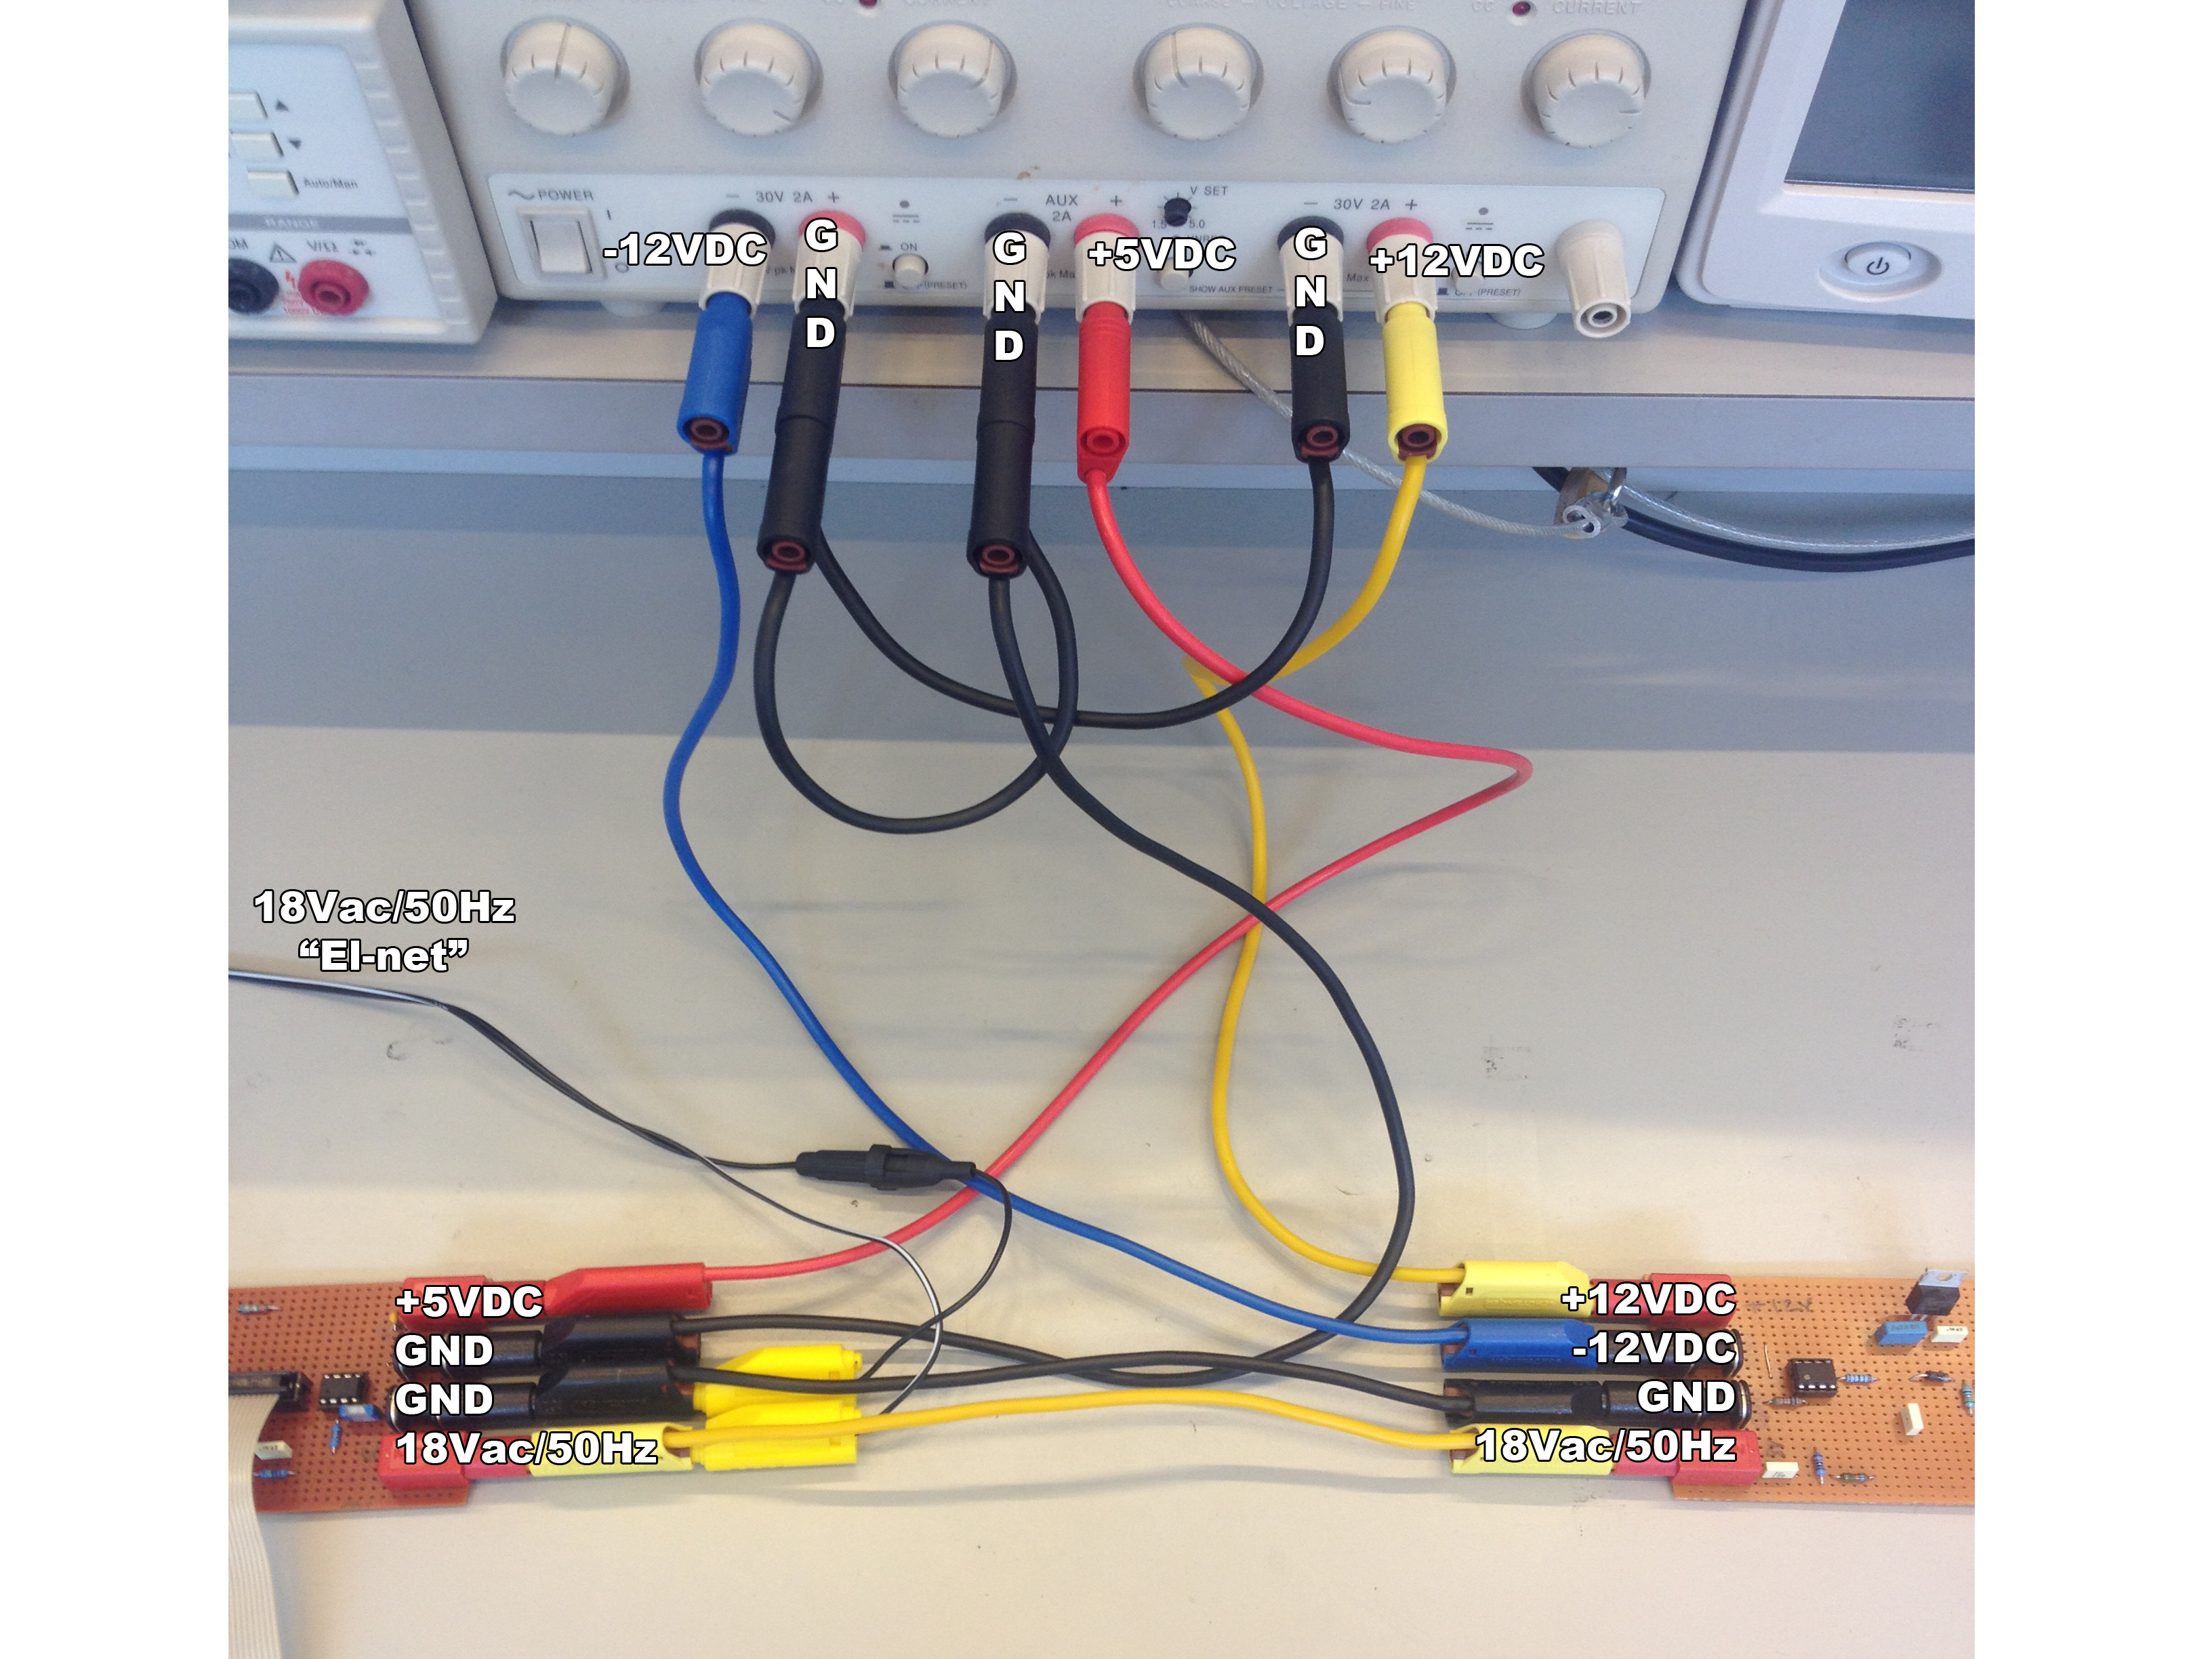
\includegraphics[width=\textwidth]{billeder/IntTest/forsyning}
	\caption{Opkobling af forsyning}
    \label{fig:opkobling_forsyning}
\end{figure}

\begin{figure}[H]
	\centering
	\includegraphics[width=0.8\textwidth]{billeder/IntTest/system}
	\caption{Overbliksbillede af samlet opsætning}
    \label{fig:system_sammensat}
\end{figure}

Spændingsforsyningen i laboratoriet har 2 variable udgange (én til venstre og én til højre), samt én fast 5VDC forsyning (midten). Begge variable udgange indstilles til 12V. 
Som det ses af figur \ref{fig:opkobling_forsyning} er + udgangen af udgangen til venstre kortsluttet med - udgangen af udgangen til højre. Dette skaber et 0 punkt, fælles ground. Herved opnås -12V i den venstre -12V udgang, samt +12V i den højre + udgang. 0 punktet forbindes til -5VDC udgangen på den faste 5VDC forsyning, for at skabe fælles ground på hele forsyningen. På encoderprintet er der skabt fælles ground mellem forsyningen og 18Vac/50Hz.

Encoderen tilsluttes +5VDC og ground.
Decoderen tilsluttes +/-12VDC.

18Vac/50Hz skaber forbindelse mellem encoder og decoder.

Hovedenhedens STK500-kit tilsluttes PC'en via en USB-til-RS232 adapter. For at PC'en kan kommunikere med microcontrolleren skal PD0 tilsluttes RDX-benet på STK500 og PD1 skal tilsluttes TDX-benet på STK500. 

Hele port D fra STK500 kittet overføres til encoderprintet. Yderligere information omkring forbinderserne i port D findes i hardwadre design for encoderen

DE2 forbindelsen til STK500 se figur \ref{fig:integration_tabel}.

\begin{figure}[H]
	\centering
	\includegraphics[width=0.6\textwidth]{billeder/IntTest/Integration_tabel}
	\caption{Forbindelsestabel}
	\label{fig:integration_tabel}
\end{figure}

\subsection{Resultat}

\begin{figure}[H]
	\centering
	\includegraphics[width=\textwidth]{billeder/IntTest/Modtager_0101_ON}
	\caption{Scopebillede af et testsignal}
	\label{fig:Modtager_0101_ON}
\end{figure}

Ovenstående figur \ref{fig:Modtager_0101_ON} viser hvad decoderen ville sende til modtager STK500 kittet. Fra PC'en er kommandoen for at aktivere udtag med adresse "0101" sendt afsted.
"1110 0101100110 01100110 000000" er den modtaget X10-kode, netop den kode som aktiverer udtaget med adresse "0101". Det er her op til modtager softwaren at arbejde med denne kode og herved sætte PD7 høj. Herved vil relæet klikke og 18Vac/50Hz udtaget er aktivt. 